\begin{frame}{Gradient Clipping}
    \begin{itemize}
        \item In case of a large or small gradient, what will happen?
        \pause
        \item Gradient descent either {\color{red} won't change our position} or will {\color{red} send us far away}.
    \end{itemize}
	\begin{figure}[H]
		\centering
		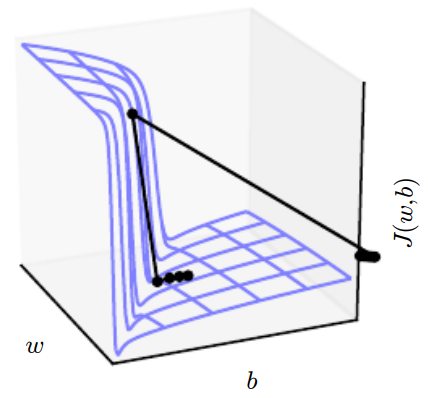
\includegraphics[width=0.4\textwidth]{Images/gard-clipping-1.png}
		\caption{The problem of large gradient value \cite{Goodfellow-et-al-2016}.}
	\end{figure}
\end{frame}

\begin{frame}{Gradient Clipping}
	\begin{itemize}
		\item Solve this problem simply by clipping gradient
		\item Clip the norm $\|\symbfit{g}\|$ of the gradient $\symbfit{g}$ before updating parameters:
		\[
		\begin{aligned}
			&\text{if} \; \|\symbfit{g}\| > v:\\
			&\qquad \symbfit{g} \gets \frac{\symbfit g}{\|\symbfit g\|} v
		\end{aligned}
		\]
		\item $v$ is the threshold for clipping which is a hyperparameter
		\item Gradient clipping saves the direction of gradient and controls its norm
	\end{itemize}
\end{frame}

\begin{frame}{Gradient Clipping}
	\begin{itemize}
		\item The effect of gradient clipping:
	\end{itemize}
	\begin{center}
		\begin{figure}[H]
			\centering
			\begin{minipage}{0.45\textwidth}
				\centering
				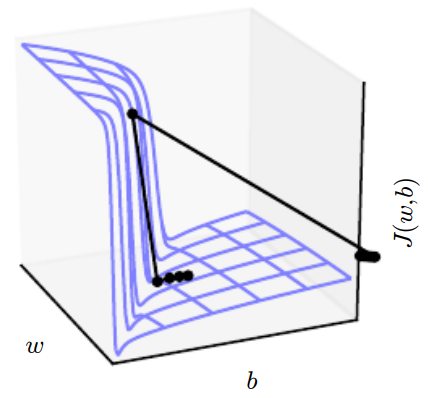
\includegraphics[width=0.8\textwidth]{Images/gard-clipping-1.png}
			\end{minipage}%\hfill
			\begin{minipage}{0.45\textwidth}
				\centering
				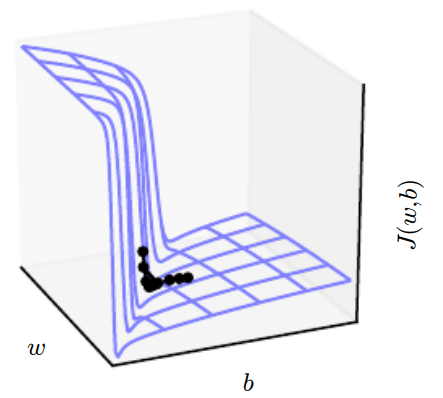
\includegraphics[width=0.8\textwidth]{Images/grad-clipping-2.png}
			\end{minipage}
			\caption{The "cliffs" landscape (left) without gradient clipping\\ and (right) with gradient clipping \cite{Goodfellow-et-al-2016}.}
		\end{figure}
	\end{center}
	
\end{frame}

\begin{frame}{Weight Initialization}
    
\end{frame}

\begin{frame}{Various GD types}
    
\end{frame}